\section{Simulation Methodology}
\label{sec:sim-method}

The objective of this section is to decompose the components of the simulation program from
high-level to low. As simulation programs are no simple task to implement, multiple modules emerge
to address specific tasks. At a systems level, these modules must then interact in such a fashion to
achieve the overall goal: avionics simulation.

An effective top-down method of presenting the taxonomy of architectures is as described in
\cite{levis_c4isr_2000}. It breaks systems down into three architectures: operational architecture, a systems architecture, and a technical architecture.

\subsection{Overview}
When describing a large piece of software, one can often decompose the software into a set of
packages. Packages describes software that are composed of multiple modules which ideally are
designed to perform a specialized task\footnote{This process can be extended ad nauseam to
further and further decompose items until its most primitive forms are derived. That will be avoided
here to keep the discussion relevant to the critical components.}. At the
subsystem level, there are three main packages: Core Avionics\footnote{Often times these modules are also referred to as
subsystems}, External Sensors and Modules, as of
course the GMSE. The modules and their interconnectivity is shown in \autoref{fig:high-level}. The
core avionics module describes the suite of software being developed that that has immediate agency
to the behavior of the avionics system. For example, the Avionics Data Computer (ADC) is the "brain"
of the avionics system. It contains the vehicle's perceived external state as well as its internal
operating state. It also supplies flow of data at the correct rate to the correct system. The Flight
Control Module (FCM) utilizes the data from the ADC to assist in maintaining stability and
controlling the vehicle to the waypoints described by the planning algorithms utilized by the
Flight Navigation Module (FNC).

For the core avionics to function in the real world, a sense of the vehicle's immediate surroundings
must be established via various sensors and external modules. In particular, the sensors (more often
than not) are an off-the-shelf product that require integration with the core avionics. The sensors
in this package may contain software modules either that mimic the behavior of a sensor, or include
the physical sensor in-the-loop of the simulation. This software package also contains "external
modules" which are other off-the-shelf components that require integration into the core avionics.
As an example, if one desires to incorporate data linking to transfer data in real-time to a base
station, the physical device to transfer the data via radio frequency (RF) would be included as an
"external module".

Lastly is the GMSE package. The objective of the GMSE package is act as the conductor by:

\begin{enumerate}
  \item spawning all the necessary processes,
  \item executing tasks at scheduled times,
  \item calculating the ``state of the world'',
  \item calculating the state of ``ownship'', and
  \item data logging and plotting.
\end{enumerate}

\begin{figure*}
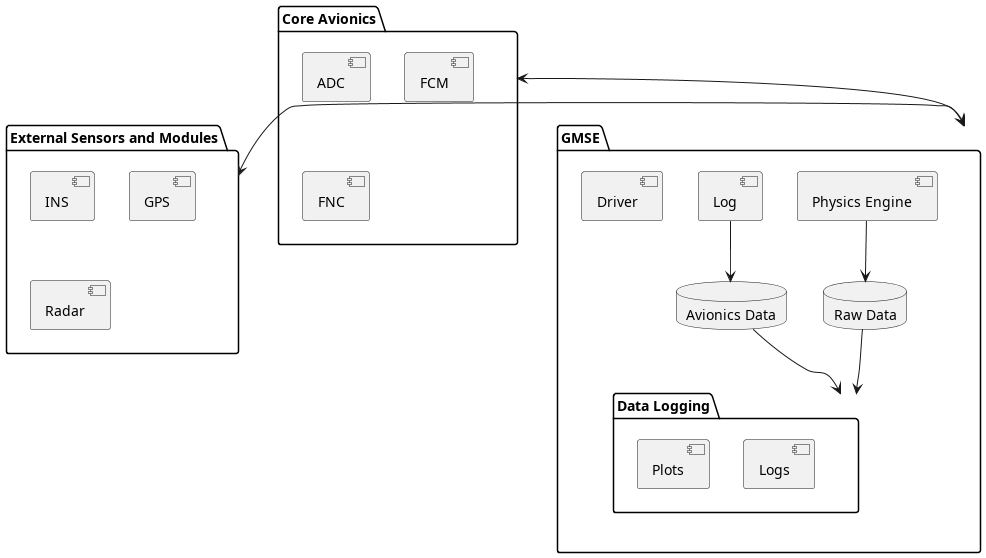
\includegraphics[width=\textwidth]{high-level}
\caption{}
\label{fig:high-level}
\end{figure*}
